\section{Activity: Pen Cap Instrument}
\subsection{Materials required}
A pen cap or marker cap
\subsection{Procedure}
Hold the pen cap by its sides. Place the open end of the cap just below your lower lip. Blow gently across the open end of the cap. Change the direction and strength of your breath until you hear a sound. Repeat the activity several times.
\newthought{Observe} Do you hear a sound? Is the pen cap moving? What is vibrating to produce the sound?
\begin{marginfigure}
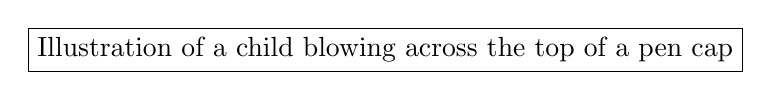
\begin{tikzpicture}
  \node[draw] at (0,0) {Illustration of a child blowing across the top of a pen cap};
\end{tikzpicture}
  \caption{Illustration of a child blowing across the top of a pen cap}
\end{marginfigure}
\subsection{Discussion}
Blowing across a pen cap produced a sound because the air inside the pen cap vibrated.